\section{Variantendiskussion}
\label{sec:Variantendiskussion}
Zu Beginn der Variantendiskussion soll eine Marktrecherche durchgeführt werden, um bestehende Lösungen zu analysieren und auf Eignung zu prüfen. Mit den gewonnen Erkenntnissen soll anschließend abgewägt werden, ob Standardsoftware beschafft werden kann oder eine Eigenentwicklung veranlasst wird.

Für eine etwaige Entwicklung sollen verschiedene Umsetzungsvarianten vorgestellt und verglichen werden, um so eine Entscheidung für das weitere Vorgehen zu treffen, welches dann im Entwurf und der Implementation umgesetzt wird.
%Das erfolgt im Rahmen einer Variantendiskussion, in der verschiedene Ansätze und Technologien zur Umsetzung der Software bewertet werden.

\subsection{Marktrecherche}
\label{sec:Marktrecherche}
Im Rahmen der Marktrecherche wurden drei verschiedene Softwarelösungen für die Anwesenheitsplanung verglichen. Das Ziel dieser Analyse war es, Akquisitionsoptionen für das geplante Softwareprojekt zu ermitteln. Um Entscheidungen über die Eignung treffen zu können, wurden die Softwareprodukte auf den Erfüllungsgrad ausgewählter Anforderungen geprüft und mit einer Bewertungsmatrix, siehe Tabelle \ref{tab:Markterkundung} bewertet. Darin enthalten sind die funktionale- und nichtfunktionale Anforderungen. Dabei wurden die Auswahlkriterien so gewählt und gewichtet, dass zwingend erforderliche Anforderungen höher gewichtet wurden als optionale Anforderungen.

%TODO:Tabelle muss ordentlich Platziert werden
\begin{table}[htbp]
    \centering
    \caption[Vergleichstabelle Markterkundung]{Tabelle Markterkundung}
    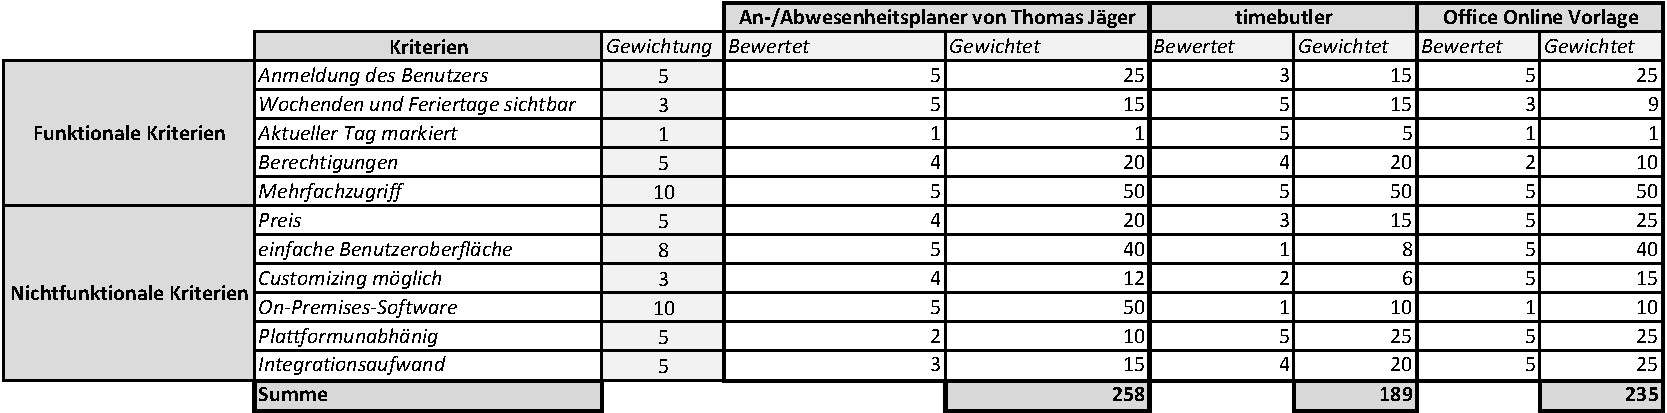
\includegraphics[width=0.9\textwidth,angle=0]{abb/Markterkundung.pdf}
    \label{tab:Markterkundung}
\end{table}

\subsubsection{An-/Abwesenheitsplaner von Thomas Jäger}
\label{sec:AnAbwesenheitsplaner}
Die erste betrachtete Software, der An-/Abwesenheitsplaner von Thomas Jäger, zeichnete sich durch die besonders intuitive Benutzeroberfläche aus. Bei der Betrachtung der funktionalen Kriterien wurde festgestellt, dass die Software alle benötigten Anforderungen erfüllt und damit für den Einsatz geeignet ist. Negativ zu bewerten, ist allerdings, dass die Software nur als Windows Programm zur Verfügung steht und damit nicht plattformunabhängig eingesetzt werden kann. Das Programm müsste auf jedem Client PC im SMK installiert werden, um die Software für alle nutzbar zu machen und wäre auf mobilen Geräten überhaut nicht verfügbar. Damit ergibt sich ein hoher initialer Integrationsaufwand und auch späterer Wartungsaufwand, welchen es zu berücksichtigen gilt. (vgl. \cite{AnAbwesenPlaner})

\subsubsection{timebutler}
\label{sec:timebutler}
Das zweite Programm namens timebutler überzeugt hingegen durch seine Plattformunabhängigkeit, da es sich um eine WebApp handelt. Damit könnte man die Software ohne großen Integrationsaufwand im SMK einführen und betreiben. Die Software bietet alle geforderten Funktionalitäten, hat jedoch eine komplizierte Benutzeroberfläche und stellt viele Funktionen bereit die nicht benötigt werden. Es resultieren höhere Anschaffungskosten als bei dem An-/Abwesenheitsplaner von Thomas Jäger. Besonders negativ ist zu bewerten, dass die Software zwar plattformunabhängig, jedoch nicht als On-Premises-Software verfügbar ist. Damit müsste auf die Cloud des Anbieters zurückgegriffen werden, was nicht wünschenswert ist. (vgl. \cite{timebutler})

\subsubsection{Online Office Datei}
\label{sec:OnlineOffice}
Die dritte zu betrachtende Lösung ist die Verwendung einer Online Office Vorlage. Diese würde es ermöglichen, die bereits vorhandenen Excel Tabellen für die Anwesenheitsplanung weiter zu verwenden. Durch das Zurückgreifen auf Online Funktionalitäten wie von Microsoft Office365 oder Onlyoffice in Verbindung mit Nextcloud kann man den gleichzeitigen Zugriff auf diese Listen erreichen. Damit würde man das Hauptproblem der einfachen Excel Dateien lösen. Doch auch hier müsste man im Falle des Einsatzes von Office365 auf die Microsoft Cloud zurückgreifen. Des Weiteren gibt es nur begrenzte Möglichkeit diese Excel Listen vor ungewollter Änderungen zu schützen und ein Berechtigungskonzept durchzusetzen.

\subsubsection{Auswertung der Marktrecherche}
\label{sec:AuswertungMarktrecherche}
Nach Betrachtung der drei Programme wurde festgestellt, dass keines der drei für eine Akquisition in frage kommt. Jedes birgt seine individuellen Schwachstellen. Der An-/Abwesenheitsplaner von Thomas Jäger wäre von allen die beste Option aufgrund der benutzerfreundliche Oberfläche, einer solide Funktionalität und einer angemessenen Preisgestaltung. Die Plattformunabhängigkeit ist jedoch im SMK ein entscheidender Faktor, da sich das neue Programm möglichst problemlos in die vorhandene Infrastruktur einfügen soll. Deswegen wurde sich gegen eine Akquisition von Standartsoftware entschieden.

Um die geforderten Funktionalitäten zu erfüllen, ohne dabei die Schwachstellen der betrachteten Programme in Kauf nehmen zu müssen, wurde die Eigenentwicklung der Software an Referat 12 übergeben. Damit soll gewährleistet werden, dass eine für da SMK optimal zugeschnittene Lösung entwickelt werden kann, sodass auch in Zukunft durch das Hinzufügen von Funktionen Aktualität gewährleistet wird.

\subsection{Eigenentwicklung}
\label{sec:Eigenentwicklung}

Durch die Eigenentwicklung sollen die spezifischen Anforderungen des SMK präzise erfüllt und so Kompromisse und Funktionslücken wie bei den verglichenen Programmen vermieden werden. Die Flexibilität und Anpassungsfähigkeit einer Eigenentwicklung ermöglicht eine perfekte Integration in bestehende Systemen im SMK. Durch den Entwurf einer an der Excel Tabelle angelehnten Benutzeroberfläche soll eine intuitive und benutzerfreundliche GUI den Umstieg der Mitarbeiter vereinfachen, was zukünftig auch den Bedarf an Schulungen reduzieren würde. Darüber hinaus führt die Eigenentwicklung zur Möglichkeit der internen Wartung und Aktualisierung. Im Nachhinein könnten einfache Funktionsupdates hinzugefügt werden, um das Anwesenheitsplanungssystem weiterzuentwickeln. Durch die Kontrolle über die genaue Funktionsweise der entwickelten Software können Datenschutz- und Datensicherheitsaspekte durch individuell implementierte Sicherheitsmaßnahmen getroffen werden.

Bei einer Eigenentwicklung ist jedoch zu beachten, dass wie bei jedem Projekt Risiken vorhanden sind. Beispielsweise ein zu hoher Zeitaufwand oder fehlendes Fachwissen könnten folgen. Diese müssen wiederum auch in der Wartung des fertigen Systems beachtet werden. Es sollte also während der Entwicklung eine Dokumentation erstellt werde, die auch andere Referatsmitglieder befähigt, die Software zu warten und \ggfs weiterzuentwickeln.


\subsection{Umsetzungsvarianten}
\label{sec:Umsetzungsvarianten}


\subsubsection{Benutzerinteraktionsmuster}
\label{sec:Benutzerinteraktionsmuster}
Nach eingehender Analyse der Anforderungen und der Markterkundung sollen verschiedene Umsetzungsvarianten für das geplante Softwareprojekt des Anwesenheitsplaners untersucht werden. Dabei soll auf bestehende Entwurfsmuster zurückgegriffen und passende ausgewählt werden. Für die Benutzerinteraktion könnte sich auf das bewährte Model-View-Controller (MVC) Entwurfsmuster gestützt werden. Dieses ermöglicht die getrennte Entwicklung von Model (Daten und Logik) und Benutzeroberfläche. Die Model-Komponente implementiert alle Funktionen, die mit Dateninteraktion und Geschäftslogik einhergehen. Die View- und die Controller-Komponente sind für alle Benutzerinteraktionen und Visualisierungsaufgaben zuständig. Der Controller bearbeitet die Benutzerinteraktionen und aktualisiert das Model, wenn das passende Event von der View ausgelöst wird. Die View wird daraufhin vom Model benachrichtigt, das Änderungen vorliegen und aktualisiert die Benutzeroberfläche anschließend mit den neuen Daten. (vgl. \cite[S. 847 - 857]{goll2011},\cite{MVC})

Als Alternative zum MVC-Muster kann auch das Model-View-ViewModel Muster (MVVM) eingesetzt werden. Es funktioniert ähnlich wie das MVC Muster mit dem Unterschied, dass die View und das ViewModel, welches die benötigten Daten aus dem Model für die View bereitstellt, direkt miteinader verbunden sind. Das ViewModel übernimmt alle für die Darstellung der View benötigten Funktionalitäten sowie die Kommunikation mit dem Model (Daten und Datenlogik). Dadurch besteht keine Verbindung zwischen View und Model mehr. Das ermöglicht eine komplette Abkopplung von Darstellung und Datenlogik.(vgl. \cite{MVVM})

\subsubsection{Systemarchitektur}
\label{sec:Systemarchitektur}
Neben der Auswahl eines Musters für die Benutzerinteraktion muss auch eine Entscheidung für eine Systemarchitektur getroffen werden. Diese bildet das Rückgrat der Anwendung und sollte daher sorgfältig gewählt werden. Es wurden insbesondere zwei Ansätze für die Entwicklung betrachtet: die monolithische Architektur und die Client-Server-Architektur.

%TODO:Monolith Quelle
Die historisch klassische Form ist die monolithische Architektur. Bei dieser entsteht ein vollkommen unabhängiges System, welches zwar mit anderen Diensten oder Datenspeichern interagiert, aber die gesamte Anwendung als Einheit bereitstellt. Das eignet sich vor allem in Fällen, in denen die Anwendung auf einer spezifischen Plattform ausgeführt werden soll und keine Notwendigkeit für eine verteilte Architektur besteht. Da die monolithische Architektur sowohl das User-Interface als auch die Logik beinhaltet, entfällt der zusätzliche Bedarf an weiteren dedizierten Servern zum Bearbeiten der Logik. Nachteil hierbei stellt die eingeschränkte Flexibilität dar, da ein solches Programm an die Plattform gebunden ist, für welche es entwickelt wurde. (vgl. \cite{Architekturen})
%TODO:QUelle Sverer Client
Die zweite betrachtete Option war die Client-Server-Architektur für Verteilte Systeme, die bei webbasierten Anwendungen oft zum Einsatz kommen. Dabei gibt es \zB bei Single-Page-Applications (SPA) ein Frontend als Benutzeroberfläche, welche von einem Backend-Server und einer Datenbank mit Daten versorgt wird. Der Backend-Server ist für die Verarbeitung der Anfragen und die Bereitstellung von Daten zuständig, während die Datenbank die persistente Speicherung der Daten ermöglicht. Der Benutzer interagiert mit der Software über das Frontend, welches die Logik beinhaltet und auf dem Client läuft. Um eine Verbindung zwischen Frontend und Backend herzustellen, sendet der Client Anfragen an den Server und erwartet entsprechende Antworten mit Daten. Die Kommunikation zwischen Client und Server erfolgt anschließend über ein Netzwerkprotokoll wie HTTP. Ein Nachteil ergibt sich dabei aus der ständige Netzwerkabhängigkeit der Clients, die zur Nutzung des Dienstes essentiell ist und ein erhöhtes Maß an Komplexität in der Entwicklung gegenüber der monolithische Architektur. (vgl. \cite{SPA})

Als Weiterentwicklung der Client-Server-Architektur kommen auch noch die Service Orientierte Architektur (SOA) und die Micro Service Architektur in Frage. Diese beiden Architekturansätze erlauben das Backend in kleinere Einzeldienste zu zerlegen, die im Anschluss unabhängig voneinander entwickelt, betrieben und skaliert werden können. Das ist ein großer Vorteil bei besonders großen Projekten, in denen verschiedene Technologien und Programmiersprachen eingesetzt werden oder ein sehr hohes Maß an Lastverteilung gefordert ist. Für Projekte mit mittlerem bis kleinem Umfang ist eine solche Architektur, jedoch nicht optimal, da das Level an Komplexität extrem steigt und die Vorteile der Architekturen wahrscheinlich nicht ausgeschöpft werden können. (vgl. \cite{SOA}, \cite{Micro})

\subsubsection{Vergleich}
\label{sec:Vergleich}
Beide der Systemarchitekturansätze kämen für den Anwesenheitsplaner in Frage. Der monolithische Ansatz könnte durch eine WPF Anwendung für Windows Clients oder einer Serverseitigen WebApp realisiert werden. Der Vorteil dabei ist, dass die Logik und die GUI direkt miteinander verbunden sind und so ein unmittelbarer Zugriff auf Benutzereingaben während der Laufzeit möglich ist. Damit benötigt man keine Schnittstellen für die Kommunikation zwischen einem Client und Server mehr. (vgl. \cite{wpf}, \cite{modernApp})

Eine Client-Server-Architektur für eine Single-Page-Application bietet sich ebenfalls an. Die Vorteile davon sind eine umfangreiche Benutzeroberfläche mit vielen Features und theoretisch geringere Netzwerkabhängigkeit, da die Anwendung auf dem Client ausgeführt wird. Im Kontext des Projektes des Anwesenheitsplaners bedeutet das, dass der Anwesenheitsplaner auf jedem Gerät im SMK auch ohne Verbindung zum Server aufgerufen werden kann, dann aber keine Daten geladen werden können. Dadurch entfällt dieser Vorteil.

Negative Aspekte bei einer Client-Server-Architektur stellen die erheblich steigende Komplexität, durch die Trennung von Frontend und Backend, dar. Es müssen Schnittstellen, \zB APIs, zur Kommunikation geschaffen werden. Um diese Nachteile auszugleichen sollten moderne Frameworks für die Entwicklung eingesetzt werden. Im Bereich der Webentwicklung ist der Kenntnisstand der Entwickler etwas geringer als bei Desktopanwendungen, was für die Umsetzung Verzögerungen bedeuten könnte. Es sollte also bei diesem Ansatz ein möglichst vertrautes Framework für die Entwicklung verwendet werden.

Ein wichtiger Faktor ist, da viele Bedienstete mit mobilen Geräten wie Smartphones und Tablets ausgestattet sind, das eine auf jedem Gerät verfügbare Anwendung entwickelt wird. Damit eignet sich eine webbasierte Anwendungen perfekt für diesen Fall. Im Gegensatz zu Desktopentwicklungen wie WPF Programme oder Smartphone Apps müssen Webanwendungen nicht installiert werden, das diese von Webservern bereitgestellt und von Browser angezeigt werden.

\subsubsection{Framework}
\label{sec:Framework}
Die Nutzung eines Frameworks für die Entwicklung ermöglicht eine effiziente Entwicklung und erleichtert die Implementierung von Architekturmustern wie \zB MVC. Bei der Auswahl sollten Aspekte wie die Verfügbarkeit von umfangreicher Dokumentation, eine aktive Entwicklergemeinschaft sowie die Integration von bewährten Bibliotheken berücksichtigt werden. Basierend auf diesen Kriterien könnten Frameworks wie Angular, React oder Vue.js in Betracht gezogen werden, die sich in der Webentwicklung bewährt haben und eine breite Unterstützung bieten. Alle diese Frameworks basieren auf Javascript und sind der Entwicklung von Single-Page-Applications angedacht. Sie benötigen geeignete Backendlösungen mit APIs als Schnittstellen sowie eine  Client-Server-Architektur. (vgl. \cite{SPA}, \cite{serverside})

Als Alternative können Frameworks wie Django, Ruby on Rails oder ASP.NET Blazor verwendet werden. Diese Frameworks ermöglichen die Erstellung von WebApps die Serverseitig laufen. Im gegensatz zu den Clientseitig laufenden WebApps werden alle Events wie \zB Klicks auf Schaltflächen auf dem Server bearbeitet werden. Der Client übermittelt nur das Event. Die Serverseite übernimmt die Verarbeitung der gesamten Logik und Datenverarbeitung inklusive des Zusammenstellens der Benutzeroberfläche, die auf der Clientseite gerendert wird. Durch diese Funktionalität kann der Zugriff auf Datenbanken oder andere Datenquellen, ohne das der Client direkten Zugriff auf diese hat, realisiert werden. Dieser Serverseitigen WebApps können sowohl als verteiltes System oder als Monolith-System aufgebaut werden. Eine wichtige Rolle bei der Wahl des Frameworks spielt die gewünschte Programmiersprache. Das Django Framework läuft mit Python, Ruby on Rails läuft mit Ruby und Blazor läuft \bzw Csharp. (vgl. \cite{BalazorServer}, \cite{serverFrameworks})

\subsubsection{Entscheidung}
\label{sec:Entscheidung}
Nach sorgfältiger Abwägung der Vor- und Nachteile der vorgestellten Umsetzungsvarianten und Architekturmuster wurde beschlossen, eine webbasierte Entwicklung und keine Desktopanwendung anzustreben, da Flexibilität und Plattformunabhänigkeit sehr wichtig für den Einsatz im SMK sind. Es soll eine WebApp entstehen, die, um Zeit und Aufwand zu minimieren, möglichst simpel aufgebaut ist. Da die Nutzerzahl selbst im Maximum unter 1000 liegt, ist eine gute Skalierbarkeit des Systems kein Faktor. Damit ist die monolithische Systemarchitektur für dieses Projekt eine gute Wahl. Um die Vorteile eines Monolithen ausnutzen zu können, sollte sich für eine Serverseitig laufende WebApp entschieden werden, da es die Fehleranfälligkeit minimiert, weil Clients keine Verbindung zu den Daten im Backend haben.

Aus den vorgestellten Frameworks für Serverseitige WebApps wurde sich gegen den Einsatz von Django und Ruby on Rails entschieden, da keine oder nur sehr wenige Erfahrungen im Umgang mit Python und Ruby vorhanden sind. Das meiste Vorwissen betrifft den Bereich der Csharp Entwicklung, weswegens auf das ASP.NET Core Blazor Framework von Microsoft gesetzt werden soll. Das Blazor Framework kann sowohl ein MVC als auch dem MVVM Modell implementieren. Damit stehen der Entwicklung beide Optionen offen.




